\documentclass{standalone}
\usepackage{tikz}
\usetikzlibrary{patterns, positioning}
\usepackage[sfdefault]{ClearSans} %% option 'sfdefault' activates Clear Sans as the default text font
\usepackage[T1]{fontenc}

\begin{document}
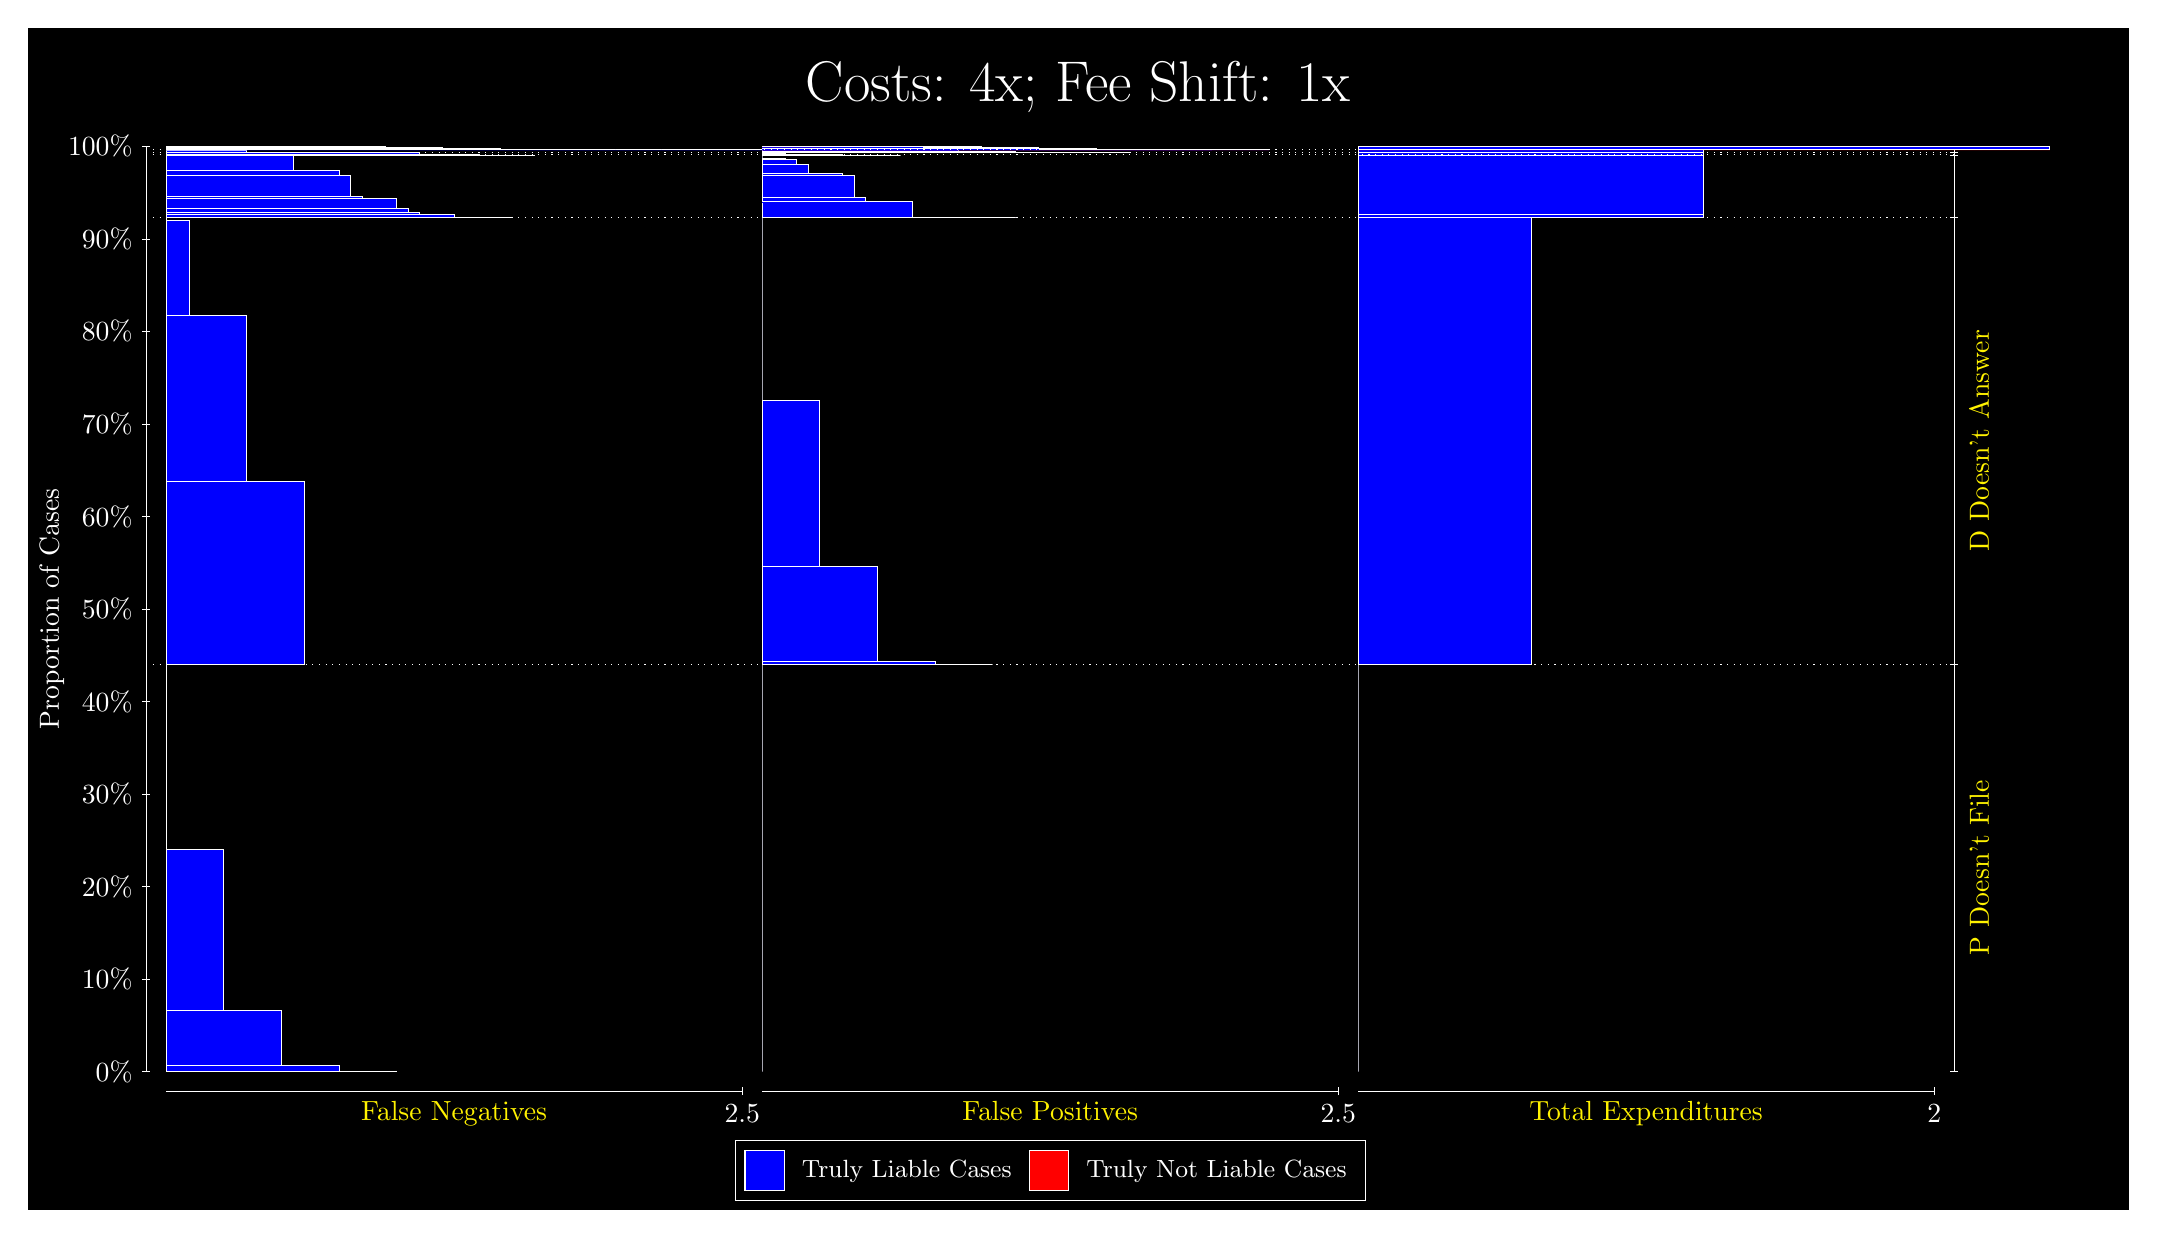
\begin{tikzpicture}
\draw[fill=black] (0,0) rectangle (26.667,15);
\draw[text=white] (0,13.5) rectangle (26.667,15) node[midway] {\huge Costs: 4x; Fee Shift: 1x};
\draw[white, very thin] (1.5,1.75) -- (1.5,13.5);
\node[rotate=90, text=white, anchor=center] at (0.3, 7.625) {Proportion of Cases};
\draw[white, very thin] (1.45,1.75) -- (1.55,1.75);
\node[text=white, anchor=east] at (1.45, 1.75) {0\%};
\draw[white, very thin] (1.45,2.925) -- (1.55,2.925);
\node[text=white, anchor=east] at (1.45, 2.925) {10\%};
\draw[white, very thin] (1.45,4.1) -- (1.55,4.1);
\node[text=white, anchor=east] at (1.45, 4.1) {20\%};
\draw[white, very thin] (1.45,5.275) -- (1.55,5.275);
\node[text=white, anchor=east] at (1.45, 5.275) {30\%};
\draw[white, very thin] (1.45,6.45) -- (1.55,6.45);
\node[text=white, anchor=east] at (1.45, 6.45) {40\%};
\draw[white, very thin] (1.45,7.625) -- (1.55,7.625);
\node[text=white, anchor=east] at (1.45, 7.625) {50\%};
\draw[white, very thin] (1.45,8.8) -- (1.55,8.8);
\node[text=white, anchor=east] at (1.45, 8.8) {60\%};
\draw[white, very thin] (1.45,9.975) -- (1.55,9.975);
\node[text=white, anchor=east] at (1.45, 9.975) {70\%};
\draw[white, very thin] (1.45,11.15) -- (1.55,11.15);
\node[text=white, anchor=east] at (1.45, 11.15) {80\%};
\draw[white, very thin] (1.45,12.325) -- (1.55,12.325);
\node[text=white, anchor=east] at (1.45, 12.325) {90\%};
\draw[white, very thin] (1.45,13.5) -- (1.55,13.5);
\node[text=white, anchor=east] at (1.45, 13.5) {100\%};

\draw[white, very thin] (24.457,1.75) -- (24.457,13.5);
\draw[white, very thin] (24.407,1.75) -- (24.507,1.75);
\node[anchor=west] at (24.407, 1.75) {};
\draw[white, very thin] (24.407,6.9194) -- (24.507,6.9194);
\node[anchor=west] at (24.407, 6.9194) {};
\draw[white, very thin] (24.407,12.601) -- (24.507,12.601);
\node[anchor=west] at (24.407, 12.601) {};
\draw[white, very thin] (24.407,13.391) -- (24.507,13.391);
\node[anchor=west] at (24.407, 13.391) {};
\draw[white, very thin] (24.407,13.425) -- (24.507,13.425);
\node[anchor=west] at (24.407, 13.425) {};
\draw[white, very thin] (24.407,13.459) -- (24.507,13.459);
\node[anchor=west] at (24.407, 13.459) {};
\draw[white, very thin] (24.407,13.5) -- (24.507,13.5);
\node[anchor=west] at (24.407, 13.5) {};

\draw[white, very thin, fill=blue] (1.75,1.75) rectangle (4.6775,1.7508);
\draw[white, very thin, fill=blue] (1.75,1.7508) rectangle (3.9457,1.828);
\draw[white, very thin, fill=blue] (1.75,1.828) rectangle (3.2138,2.5217);
\draw[white, very thin, fill=blue] (1.75,2.5217) rectangle (2.4819,4.5724);
\draw[white, very thin, fill=red] (1.75,4.5724) rectangle (1.75,4.5724);
\draw[white, very thin, fill=blue] (1.75,4.5724) rectangle (1.75,6.9194);
\draw[white, very thin, fill=blue] (1.75,6.9194) rectangle (3.5065,9.2472);
\draw[white, very thin, fill=blue] (1.75,9.2472) rectangle (2.7746,11.355);
\draw[white, very thin, fill=blue] (1.75,11.355) rectangle (2.0428,12.559);
\draw[white, very thin, fill=red] (1.75,12.559) rectangle (1.75,12.559);
\draw[white, very thin, fill=blue] (1.75,12.559) rectangle (1.75,12.601);
\draw[white, very thin, fill=blue] (1.75,12.601) rectangle (6.1413,12.601);
\draw[white, very thin, fill=blue] (1.75,12.601) rectangle (5.5558,12.603);
\draw[white, very thin, fill=blue] (1.75,12.603) rectangle (5.4094,12.643);
\draw[white, very thin, fill=blue] (1.75,12.643) rectangle (4.9703,12.66);
\draw[white, very thin, fill=blue] (1.75,12.66) rectangle (4.8239,12.716);
\draw[white, very thin, fill=blue] (1.75,12.716) rectangle (4.6775,12.836);
\draw[white, very thin, fill=blue] (1.75,12.836) rectangle (4.2384,12.86);
\draw[white, very thin, fill=blue] (1.75,12.86) rectangle (4.092,13.134);
\draw[white, very thin, fill=blue] (1.75,13.134) rectangle (3.9457,13.195);
\draw[white, very thin, fill=blue] (1.75,13.195) rectangle (3.5065,13.196);
\draw[white, very thin, fill=blue] (1.75,13.196) rectangle (3.3602,13.388);
\draw[white, very thin, fill=blue] (1.75,13.388) rectangle (3.2138,13.389);
\draw[white, very thin, fill=blue] (1.75,13.389) rectangle (2.7746,13.389);
\draw[white, very thin, fill=blue] (1.75,13.389) rectangle (2.6283,13.391);
\draw[white, very thin, fill=blue] (1.75,13.391) rectangle (2.0428,13.391);
\draw[white, very thin, fill=red] (1.75,13.391) rectangle (1.75,13.391);
\draw[white, very thin, fill=blue] (1.75,13.391) rectangle (6.4341,13.391);
\draw[white, very thin, fill=blue] (1.75,13.391) rectangle (5.7022,13.404);
\draw[white, very thin, fill=blue] (1.75,13.404) rectangle (4.9703,13.423);
\draw[white, very thin, fill=blue] (1.75,13.423) rectangle (4.2384,13.425);
\draw[white, very thin, fill=blue] (1.75,13.425) rectangle (3.5065,13.425);
\draw[white, very thin, fill=red] (1.75,13.425) rectangle (1.75,13.425);
\draw[white, very thin, fill=blue] (1.75,13.425) rectangle (3.5065,13.426);
\draw[white, very thin, fill=blue] (1.75,13.426) rectangle (2.7746,13.445);
\draw[white, very thin, fill=blue] (1.75,13.445) rectangle (2.0428,13.459);
\draw[white, very thin, fill=red] (1.75,13.459) rectangle (1.75,13.459);
\draw[white, very thin, fill=blue] (1.75,13.459) rectangle (1.75,13.459);
\draw[white, very thin, fill=blue] (1.75,13.459) rectangle (11.704,13.459);
\draw[white, very thin, fill=blue] (1.75,13.459) rectangle (10.972,13.459);
\draw[white, very thin, fill=blue] (1.75,13.459) rectangle (10.24,13.46);
\draw[white, very thin, fill=blue] (1.75,13.46) rectangle (9.508,13.463);
\draw[white, very thin, fill=blue] (1.75,13.463) rectangle (8.7761,13.464);
\draw[white, very thin, fill=blue] (1.75,13.464) rectangle (8.0442,13.464);
\draw[white, very thin, fill=blue] (1.75,13.464) rectangle (7.4587,13.464);
\draw[white, very thin, fill=blue] (1.75,13.464) rectangle (6.7268,13.464);
\draw[white, very thin, fill=blue] (1.75,13.464) rectangle (5.9949,13.47);
\draw[white, very thin, fill=blue] (1.75,13.47) rectangle (5.2631,13.49);
\draw[white, very thin, fill=blue] (1.75,13.49) rectangle (4.5312,13.499);
\draw[white, very thin, fill=blue] (1.75,13.499) rectangle (3.7993,13.5);
\draw[white, very thin, fill=blue] (1.75,13.5) rectangle (3.0674,13.5);
\draw[white, very thin, fill=blue] (1.75,13.5) rectangle (2.3355,13.5);
\draw[white, very thin, fill=red] (1.75,13.5) rectangle (1.75,13.5);
\draw[white, very thin, fill=red] (9.3189,1.75) rectangle (9.3189,1.75);
\draw[white, very thin, fill=blue] (9.3189,1.75) rectangle (9.3189,6.9194);
\draw[white, very thin, fill=red] (9.3189,6.9194) rectangle (12.246,6.9194);
\draw[white, very thin, fill=blue] (9.3189,6.9194) rectangle (12.246,6.9194);
\draw[white, very thin, fill=blue] (9.3189,6.9194) rectangle (11.515,6.9609);
\draw[white, very thin, fill=blue] (9.3189,6.9609) rectangle (10.783,8.1647);
\draw[white, very thin, fill=blue] (9.3189,8.1647) rectangle (10.051,10.273);
\draw[white, very thin, fill=blue] (9.3189,10.273) rectangle (9.3189,12.601);
\draw[white, very thin, fill=red] (9.3189,12.601) rectangle (12.539,12.601);
\draw[white, very thin, fill=blue] (9.3189,12.601) rectangle (12.539,12.601);
\draw[white, very thin, fill=red] (9.3189,12.601) rectangle (11.954,12.601);
\draw[white, very thin, fill=blue] (9.3189,12.601) rectangle (11.954,12.603);
\draw[white, very thin, fill=blue] (9.3189,12.603) rectangle (11.807,12.603);
\draw[white, very thin, fill=red] (9.3189,12.603) rectangle (11.368,12.603);
\draw[white, very thin, fill=blue] (9.3189,12.603) rectangle (11.368,12.603);
\draw[white, very thin, fill=blue] (9.3189,12.603) rectangle (11.222,12.796);
\draw[white, very thin, fill=blue] (9.3189,12.796) rectangle (11.075,12.797);
\draw[white, very thin, fill=blue] (9.3189,12.797) rectangle (10.636,12.858);
\draw[white, very thin, fill=blue] (9.3189,12.858) rectangle (10.49,13.131);
\draw[white, very thin, fill=blue] (9.3189,13.131) rectangle (10.344,13.156);
\draw[white, very thin, fill=blue] (9.3189,13.156) rectangle (9.9044,13.276);
\draw[white, very thin, fill=blue] (9.3189,13.276) rectangle (9.758,13.331);
\draw[white, very thin, fill=blue] (9.3189,13.331) rectangle (9.6116,13.348);
\draw[white, very thin, fill=blue] (9.3189,13.348) rectangle (9.3189,13.391);
\draw[white, very thin, fill=red] (9.3189,13.391) rectangle (11.075,13.391);
\draw[white, very thin, fill=blue] (9.3189,13.391) rectangle (11.075,13.391);
\draw[white, very thin, fill=blue] (9.3189,13.391) rectangle (10.344,13.394);
\draw[white, very thin, fill=blue] (9.3189,13.394) rectangle (9.6116,13.412);
\draw[white, very thin, fill=blue] (9.3189,13.412) rectangle (9.3189,13.425);
\draw[white, very thin, fill=red] (9.3189,13.425) rectangle (14.003,13.425);
\draw[white, very thin, fill=blue] (9.3189,13.425) rectangle (14.003,13.425);
\draw[white, very thin, fill=blue] (9.3189,13.425) rectangle (13.271,13.426);
\draw[white, very thin, fill=blue] (9.3189,13.426) rectangle (12.539,13.44);
\draw[white, very thin, fill=blue] (9.3189,13.44) rectangle (11.807,13.459);
\draw[white, very thin, fill=blue] (9.3189,13.459) rectangle (11.075,13.459);
\draw[white, very thin, fill=red] (9.3189,13.459) rectangle (15.759,13.459);
\draw[white, very thin, fill=blue] (9.3189,13.459) rectangle (15.759,13.459);
\draw[white, very thin, fill=blue] (9.3189,13.459) rectangle (15.028,13.459);
\draw[white, very thin, fill=red] (9.3189,13.459) rectangle (15.028,13.459);
\draw[white, very thin, fill=blue] (9.3189,13.459) rectangle (15.028,13.459);
\draw[white, very thin, fill=blue] (9.3189,13.459) rectangle (14.296,13.46);
\draw[white, very thin, fill=red] (9.3189,13.46) rectangle (14.296,13.46);
\draw[white, very thin, fill=blue] (9.3189,13.46) rectangle (14.296,13.46);
\draw[white, very thin, fill=blue] (9.3189,13.46) rectangle (13.564,13.463);
\draw[white, very thin, fill=red] (9.3189,13.463) rectangle (13.564,13.463);
\draw[white, very thin, fill=blue] (9.3189,13.463) rectangle (13.564,13.469);
\draw[white, very thin, fill=blue] (9.3189,13.469) rectangle (12.832,13.47);
\draw[white, very thin, fill=blue] (9.3189,13.47) rectangle (12.832,13.489);
\draw[white, very thin, fill=blue] (9.3189,13.489) rectangle (12.1,13.495);
\draw[white, very thin, fill=blue] (9.3189,13.495) rectangle (11.368,13.496);
\draw[white, very thin, fill=blue] (9.3189,13.496) rectangle (10.636,13.496);
\draw[white, very thin, fill=red] (9.3189,13.496) rectangle (10.051,13.496);
\draw[white, very thin, fill=blue] (9.3189,13.496) rectangle (10.051,13.496);
\draw[white, very thin, fill=red] (9.3189,13.496) rectangle (9.3189,13.496);
\draw[white, very thin, fill=blue] (9.3189,13.496) rectangle (9.3189,13.5);
\draw[white, very thin, fill=red] (16.888,1.75) rectangle (16.888,1.75);
\draw[white, very thin, fill=blue] (16.888,1.75) rectangle (16.888,6.9194);
\draw[white, very thin, fill=red] (16.888,6.9194) rectangle (19.083,6.9194);
\draw[white, very thin, fill=blue] (16.888,6.9194) rectangle (19.083,12.601);
\draw[white, very thin, fill=red] (16.888,12.601) rectangle (21.279,12.601);
\draw[white, very thin, fill=blue] (16.888,12.601) rectangle (21.279,12.643);
\draw[white, very thin, fill=red] (16.888,12.643) rectangle (21.279,12.643);
\draw[white, very thin, fill=blue] (16.888,12.643) rectangle (21.279,13.391);
\draw[white, very thin, fill=red] (16.888,13.391) rectangle (21.279,13.391);
\draw[white, very thin, fill=blue] (16.888,13.391) rectangle (21.279,13.425);
\draw[white, very thin, fill=red] (16.888,13.425) rectangle (21.279,13.425);
\draw[white, very thin, fill=blue] (16.888,13.425) rectangle (21.279,13.459);
\draw[white, very thin, fill=red] (16.888,13.459) rectangle (25.67,13.459);
\draw[white, very thin, fill=blue] (16.888,13.459) rectangle (25.67,13.463);
\draw[white, very thin, fill=red] (16.888,13.463) rectangle (25.67,13.463);
\draw[white, very thin, fill=blue] (16.888,13.463) rectangle (25.67,13.5);
\draw[white, dotted] (1.5,6.9194) -- (24.457,6.9194);
\draw[white, dotted] (1.5,12.601) -- (24.457,12.601);
\draw[white, dotted] (1.5,13.391) -- (24.457,13.391);
\draw[white, dotted] (1.5,13.425) -- (24.457,13.425);
\draw[white, dotted] (1.5,13.459) -- (24.457,13.459);
\draw[white, very thin] (1.75,1.5) -- (9.0689,1.5);
\node[text=yellow, anchor=north] at (5.4094, 1.5) {False Negatives};
\draw[white, very thin] (9.0689,1.45) -- (9.0689,1.55);
\node[text=white, anchor=north] at (9.0689, 1.45) {2.5};

\draw[white, very thin] (9.3189,1.5) -- (16.638,1.5);
\node[text=yellow, anchor=north] at (12.978, 1.5) {False Positives};
\draw[white, very thin] (16.638,1.45) -- (16.638,1.55);
\node[text=white, anchor=north] at (16.638, 1.45) {2.5};

\draw[white, very thin] (16.888,1.5) -- (24.207,1.5);
\node[text=yellow, anchor=north] at (20.547, 1.5) {Total Expenditures};
\draw[white, very thin] (24.207,1.45) -- (24.207,1.55);
\node[text=white, anchor=north] at (24.207, 1.45) {2};

\node[text=yellow, centered, rotate=90] at (24.777, 4.3347) {P Doesn't File};
\node[text=yellow, centered, rotate=90] at (24.777, 9.76) {D Doesn't Answer};





\draw (12.978300999999998,1.5) node[draw=none] (baseCoordinate) {};
\begin{scope}[align=center]
        \matrix[scale=0.5, draw=white, below=0.5cm of baseCoordinate, nodes={draw}, column sep=0.1cm]{
            \node[rectangle, draw, minimum width=0.5cm, minimum height=0.5cm, fill=blue] {}; &
            \node[draw=none, font=\small, text=white] (B) {Truly Liable Cases}; &
            \node[rectangle, draw, minimum width=0.5cm, minimum height=0.5cm, fill=red] {}; &
            \node[draw=none, font=\small, text=white] (B) {Truly Not Liable Cases}; \\
            };
\end{scope}

\end{tikzpicture}
\end{document}